% A Tale of Two Slinkies: Learning about Model Building in a Student Driven Classroom
%
% Calvin Berggren, Punit Gandhi, Jesse Livezey, Ryan Olf
%
% 2013-08-??: v1
%
\documentclass[pre,preprint,superscriptaddress,longbibliography]{revtex4-1} 
%\documentclass[pre,superscriptaddress,twocolumn]{revtex4-1} 
\usepackage{graphicx}
\usepackage{hyperref}
\usepackage{amsmath}
\usepackage{amsfonts} % needed for bold Greek, Fraktur, and blackboard bold
\usepackage{amssymb}
\usepackage[margin=1in]{geometry}
\usepackage{dcolumn}
\usepackage{multirow}
\usepackage{tikz}
\usetikzlibrary{calc,patterns,decorations.pathmorphing,decorations.markings}

% TODO: remove these lines, which expand the margins (useful for comments)
%\textwidth  .72\paperwidth
%\hoffset -1in
%\oddsidemargin .14\paperwidth
%\evensidemargin .14\paperwidth
%\marginparwidth .11\paperwidth


% Draft macros
%\usepackage[normalem]{ulem} % for strikethrough
%\usepackage[usenames,dvipsnames]{xcolor}
%\newcommand{\TODO}[1]{\marginpar{\raggedright\scriptsize\textbf{TODO:} #1} (\textbf{TODO})}
%\newcommand{\NOTEMARG}[1]{\marginpar{\raggedright\scriptsize\textbf{NOTE:} #1} (\textbf{NOTE})}
%\newcommand{\NOTE}[1]{\marginpar{\footnotesize\textbf{NOTE}} (\textbf{NOTE: #1})}
%\definecolor{purple}{rgb}{1,0,1}
%\newcommand{\calvin}[2]{\textcolor{purple}{\sout{#1}#2}}

\newcommand{\eq}[1]{eq.~\eqref{eq:#1}}
\newcommand{\eqs}[2]{eqs.~\eqref{eq:#1} and \eqref{eq:#2}}
\renewcommand{\sec}[1]{section~\ref{sec:#1}}
\newcommand{\secs}[2]{sections~\ref{sec:#1} and \ref{sec:#2}}
\newcommand{\subsec}[1]{section~\ref{subsec:#1}}
\newcommand{\subsubsec}[1]{section~\ref{subsubsec:#1}}
\newcommand{\app}[1]{appendix~\ref{app:#1}}
\newcommand{\fig}[1]{figure~\ref{fig:#1}}
\newcommand{\figs}[2]{figures~\ref{fig:#1} and \ref{fig:#2}}
\newcommand{\tab}[1]{table~\ref{tab:#1}}
\newcommand{\nn}{\nonumber}



\newcommand{\TABcurriculum}{
\begin{table}[h]\centering
\begin{tabular}{c|c|c}
Compare falling slinkies to falling rigid objects & 4 hours & Newton's 2nd law, gravity\\
Mass and spring model & 7 hours & Hooke's Law, discrete approximation, numerical simulation\\
Wave model &  7 hours & Wave propagation \\
Final projects & 10 hours &

\end{tabular}
\caption{\label{tab:curriculum} An brief overview of the curriculum of the week-long program.}
\end{table}
}

\newcommand{\FIGstudents}{
\begin{figure}[t]\center
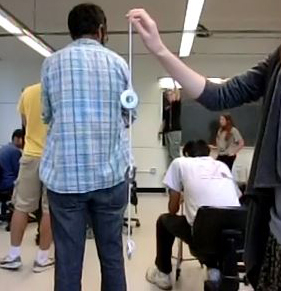
\includegraphics[width=\columnwidth]{./img/students_small.jpg}
\caption{\label{fig:students} Students from a recent Compass Project summer program testing model slinkies built out of washers and rubberbands.}
\end{figure}
}

\newcommand{\FIGdiscrete}{
\begin{figure}[t]\center
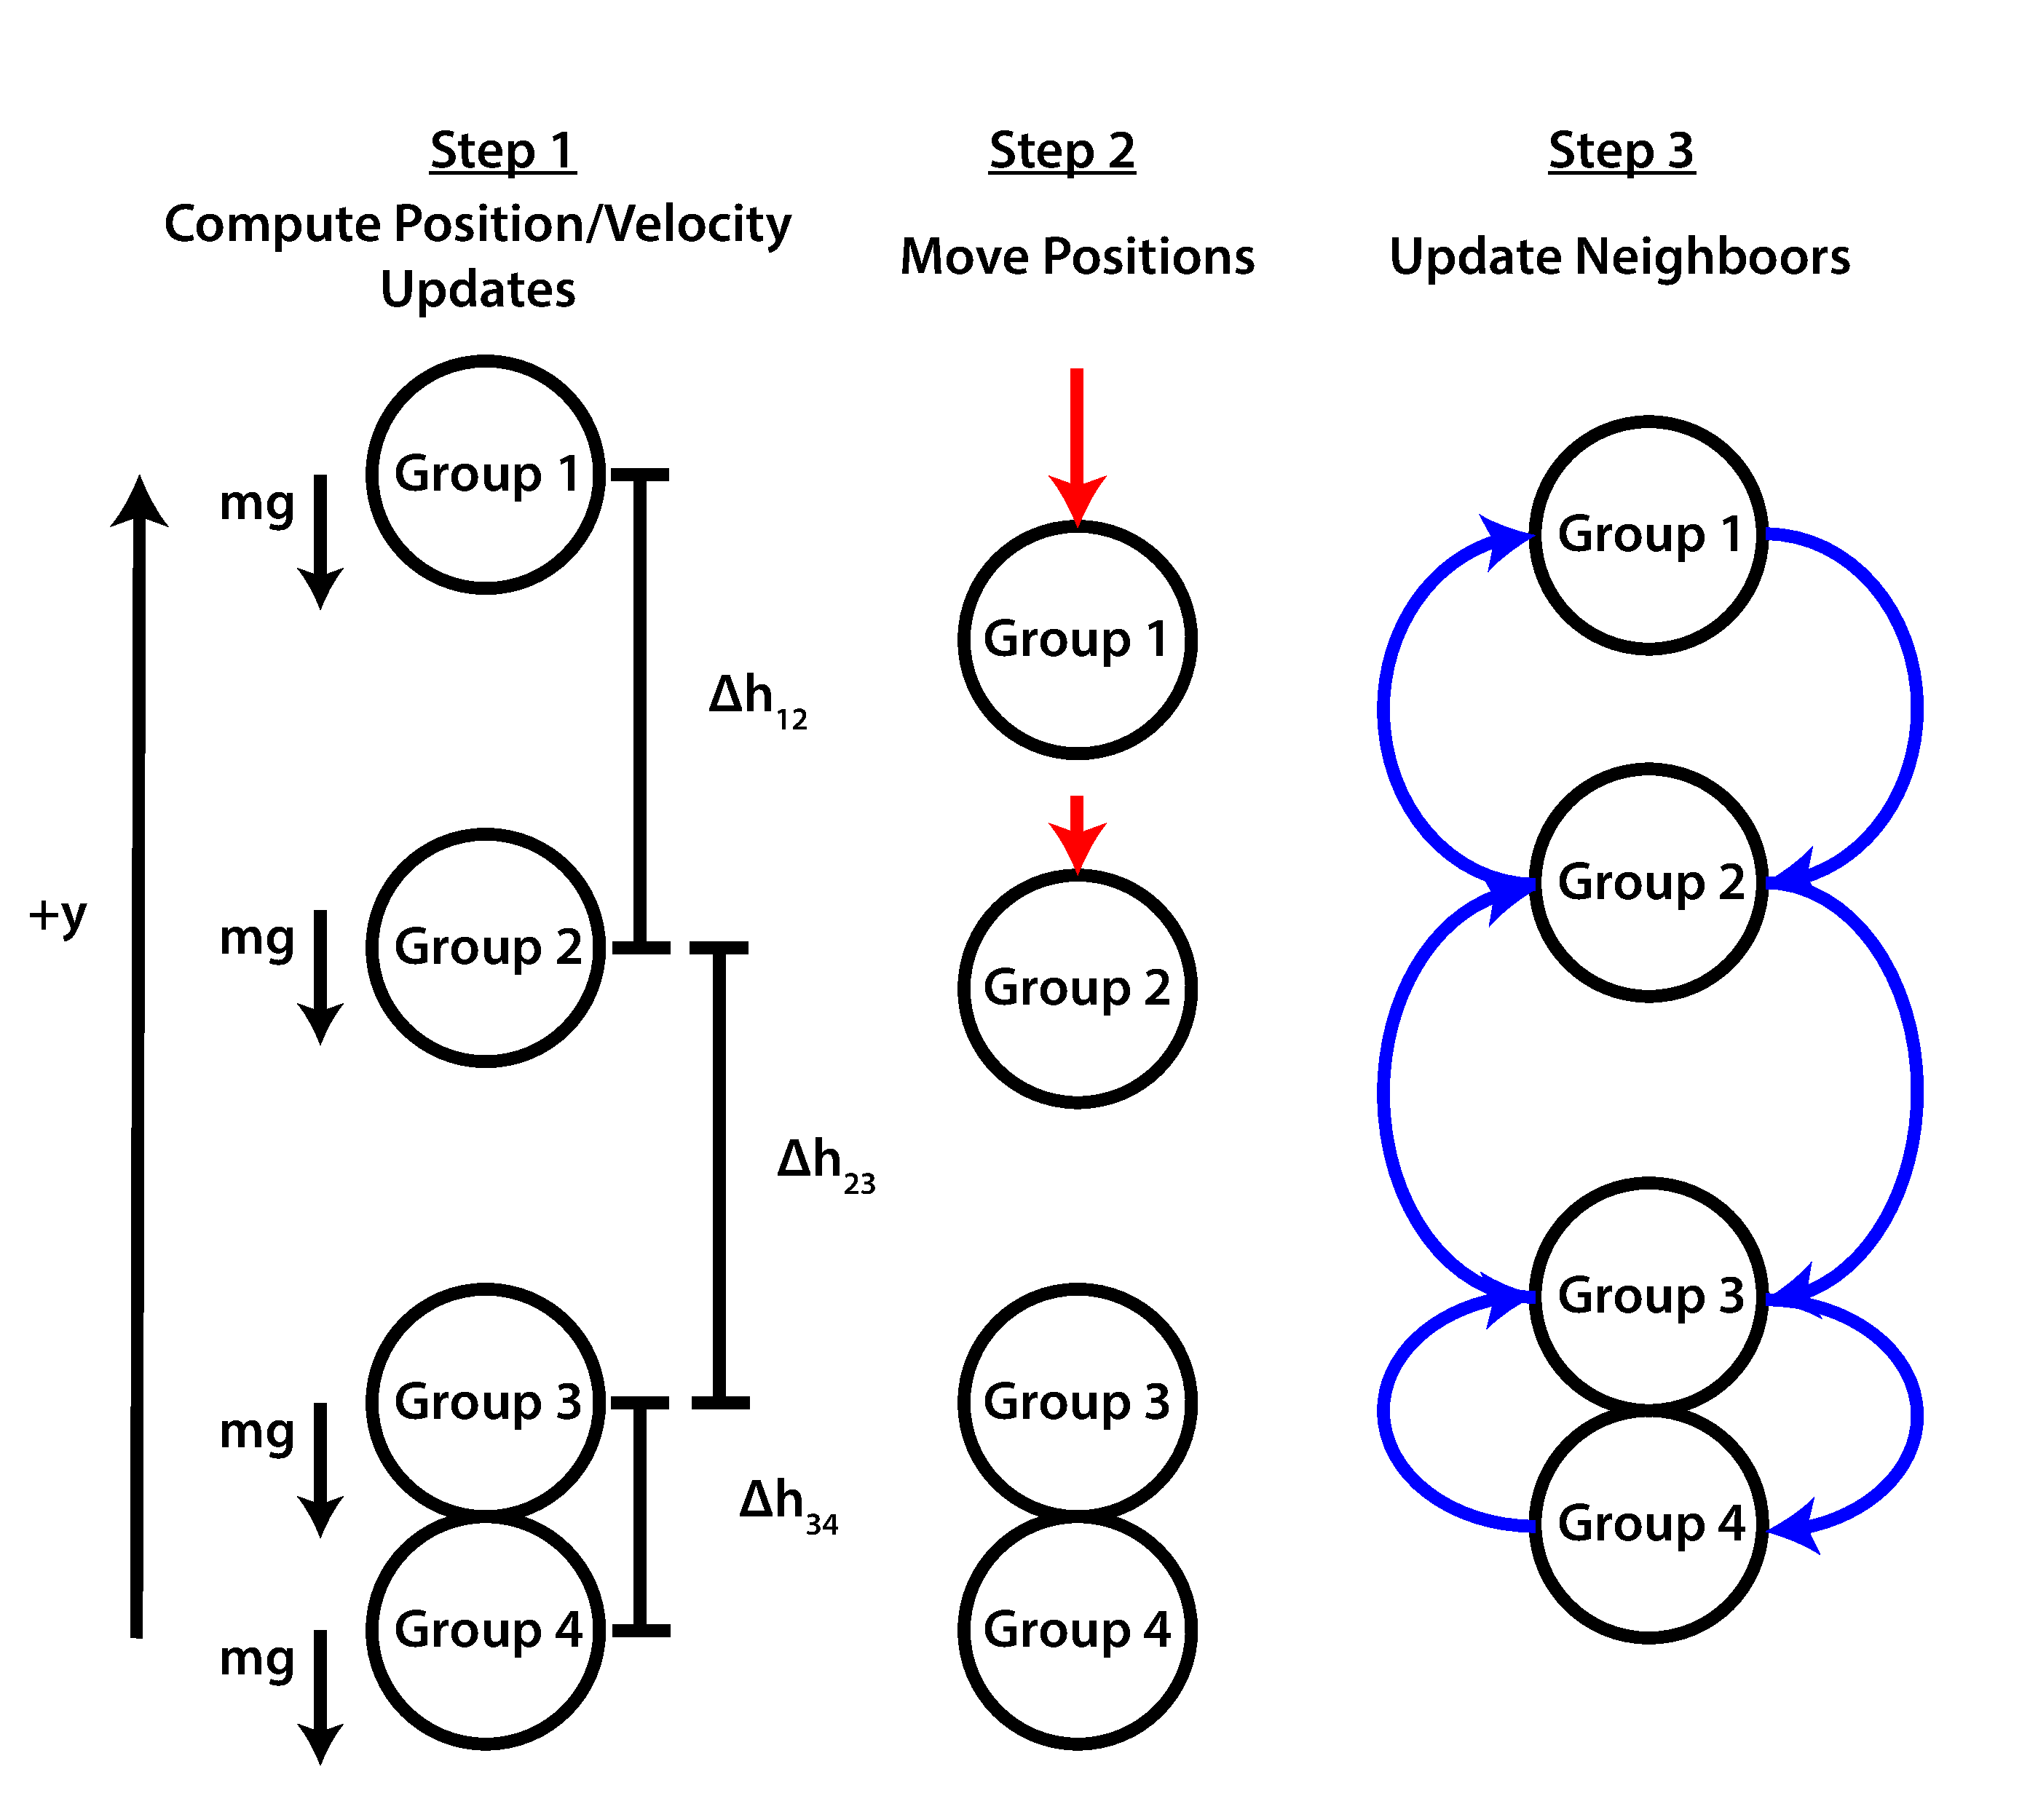
\includegraphics[width=\columnwidth]{./img/discrete_model.pdf}
\caption{\label{fig:discrete} \textbf{Should this be from class simulation?  Should we plot something else, or something different to maybe show parameter dependence?}Vertical position of the four masses with mass $m=$ as a function of time for a simulation of the discrete model with timestep $\Delta t=$, spring constant $k=$.  \textbf{Add photo showing class "simulation"?}}
\end{figure}
}

\newcommand{\FIGclumppulse}{
\begin{figure}[t]\center
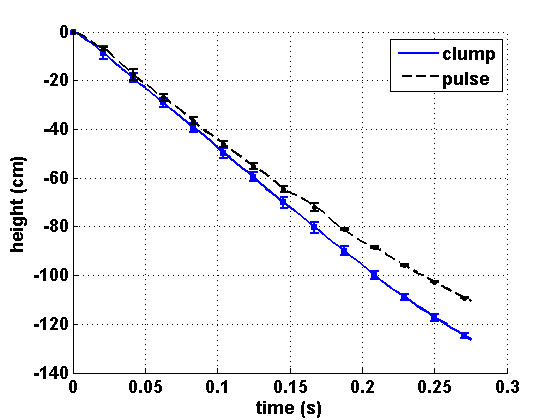
\includegraphics[width=\columnwidth]{./img/ClumpPulse.png}
\caption{\label{fig:clumppulse} A few frames from a slow motion image of a wave pulse sent down a slinky next to a falling slinky,\textbf{Add frames} and a graph of position vs time of the top of the falling slinky and the wave pulse.}
\end{figure}
}


\begin{document}

\title{A Tale of Two Slinkies: Learning about Model Building in a Student-Driven Classroom}
\author{Punit  Gandhi}
\email{punit\_gandhi@berkeley.edu}
\affiliation{Department of Physics, University of California, Berkeley, CA 94720, USA}
\author{Ryan Olf}
%\email{ryanolf@berkeley.edu}
\affiliation{Department of Physics, University of California, Berkeley, CA 94720, USA}
\author{Jesse Livezey}
\affiliation{Department of Physics, University of California, Berkeley, CA 94720, USA}
\affiliation{Redwood Center for Theoretical Neuroscience, University of California at Berkeley, Berkeley, CA 94720, USA}
%\email{jesse.livezey@berkeley.edu}
\author{Calvin Berggren}
%\email{calvin1414@berkeley.edu}
\affiliation{Department of Physics, Texas Lutheran University, Seguin, TX 78154}
\date{\today}

\maketitle

We describe a set of conceptual  and hands-on activities based around understanding the dynamics of a slinky that is hung vertically and released from rest.  
This slinky drop experiment typically lasts a fraction of a second, but when observed in slow motion one sees the slinky compress from the top down while the bottom portion remains at rest\footnote{We note that the bottom of the slinky does not remain completely at rest, but actually twists before the collapse completes.  A phenomena that was explored by one of the groups as a final project.}---naively seeming to defy gravity---until the slinky has completed its collapse.  The motion, or lack thereof, of the bottom of the slinky after the top is dropped is meant to spark student curiosity by challenging  expectations and providing motivation and context for learning about scientific model building. 



The slinky drop  and other related phenomena have been studied in detail\cite{calkin1993, newburgh1995, graham2001, aguirregabiria2007,unruh2011, cross2012} and have attracted a flurry of interest online \cite{..}. The slinky drop  can be understood in terms of two distinct models that are both accessible to students and provide complementary insight: a discrete mass model and a continuous wave model.  
%In this work, we describe how we used the slinky drop phenomenon to teach the modeling process by giving the students first-hand experience constructing two distinct but complementary physical models.
 The sequence of activities we present were developed as a part of a week-long summer program for incoming freshmen through the Compass Project,~\cite{albana2013,Roth2012,drdf2013a,drdf2013b,gandhi2014} but could easily be implemented in a wide range of classrooms at the high school and introductory college levels.   % By engaging 

After providing a brief overview of curriculum and the classroom setting in which it was implented, we describe the key activities that allowed the students to explore each of the two models that provide insight into how the slinky seems to defy gravity.   

\section{Curriculum Overview}

 

%Students in the class shared a common interest in the physical sciences but came from diverse backgrounds with widely varying levels of preparation. %In spite of this, it was important that all students be able to contribute to and take ownership of the models developed in the course. 
%The slinky drop phenomenon strikes a delicate balance between competing pedagogical needs. The setup is simple enough that even less prepared students have (incorrect) intuition for what should happen, and can therefore be surprised by the observed (contradictory) result.  %, which engages the students interest and motivates further exploration. 
%On the other hand, a satisfactory intuitive understanding of the phenomenon is both attainable to a wide range of students and  sufficiently\textbf{•} challenging that such students can begin their exploration on a relatively level playing field.%, facilitating collaboration and shared learning. 
Paragraph for why slinky drop is good

(1) its wierd and don't need much background to see
(2) basic physics tools + nuanced modeling + easily realizable experimentally

nontrivial models can be built out of basic physics tools.


We note that this curriculum does not explicitly rely on previous physics knowledge from the students, and all the concepts from Newton's laws to wave propagation were introduced in a self-contained way in a collaborative learning environment that blends several proven inquiry- and discovery-based strategies, such as \emph{Complex Instruction}~\cite{Cohen1997}, \emph{Constructionism}~\cite{Papert1991}, and \emph{Modeling Discourse Management}~\cite{Desbien2002} (an implementation of \emph{Modeling Instruction}~\cite{Brewe2008}).   The material was presented with an emphasis on building intuition and experimentally verifying the relevant physics principles, and thus proved challenging even for those with a previous physics background.  The curriculum, outlined in Table~\ref{tab:curriculum}, consists of four major parts and was implemented with 16 students over a total of about 30 hours of instruction spread over 7 days. The students additionally spent approximately 10 hours on group homework assignments. 

In the first part of the course, the students reconciled their observations of the levitating slinky with their existing intuition about gravity based on point objects.  By dropping a small ball next to a vertically hung slinky that is simultaneously released, the students found a particular initial height relative to the top of the slinky for the ball such that ball and slinky hit the floor at the same time\footnote{Connecting this experiment to the concept of center of mass was the subject of a final project}.
%After first exploring how gravity acts on extended objects  to convince themselves that the slinky doesn't actually defy gravity, students approached the slinky drop problem using two complementary models. 
%In one approach, detailed in \sec{sec:forces}, students 
The students then approximated the slinky as a finite number of point masses connected by linear massless springs, allowing them to apply  Newton's Laws to calculate the motion of the masses  (Sec.~\ref{sec:discrete})  and gain insight into the slinky drop problem.  
Observations made during the exploration of this model motivate a second approach, wherein students modeled the propagation of information in the slinky (Sec.~\ref{sec:wave}). This model describes the event when the slinky is released as a piece of information that needs to travel to other parts of the system---via either a wave pulse or the shock wave of medium collapse---before they are able to respond.  ``Information'' initially proved to be a more challenging concept for the students to grasp but ultimately provided a clearer, more intuitive way of understanding why the bottom remains stationary.  %The bottom of the slinky remains stationary because it does not know the top has been released.  
The fourth and final phase of the curriculum was group research projects where the students chose to explore a question related to the slinky phenomena in depth and create a youtube style video explaining their results for a general audience~\cite{compassyoutube}. 

\TABcurriculum


\section{A discrete mass and spring  model of the slinky}
\label{sec:discrete}
In this model (the ``discrete model''), students used forces and Newton's Laws to calculate the
motion of the slinky in free fall. This
model is conceptually straightforward and allowed students to follow a
reductionist approach wherein they divide the slinky into intuitively and mathematically accessible
constituents. In particular, students broke the model slinky into a series of point masses connected by massless springs that obey Hooke's Law.%,as shown in \fig{discrete}.
% The equations of motion that result from this simple model are quite difficult to solve analytically for slinkies composed of more than a few masses, but the model is still very useful in understanding the slinky drop in particular, and model building in general. 

The students faced many choices regarding approximations and simplifications with the goal of making the analysis tractable while still capturing the phenomenon of interest. %Which choices that render the mathematics more tractable, such as choosing to model only a few masses, yield a system that reproduces the levitating slinky phenomenon? 
In order to glean insight into the slinky drop, they investigated the roles that various parameters of the model---number, mass, spring constant---play in reproducing the relevant qualities of a slinky.  The students explored the model in two complementary ways: in Sec. \ref{sec:discrete:exp} they built and studied a physical approximation of the discrete system, while in Sec. \ref{sec:discrete:num} they numerically evolved the derived equations of motion.

\subsection{experimental exploration}
\label{sec:discrete:exp}
%In order to be useful for understanding the the slinky drop, the discrete model needs to be able to reproduce the essential physics of the slinky. 
The students explored the applicability and limitations of the discrete model, and the implications of the various choices involved in defining it, by building physical realizations of the model using masses (washers, nuts) tied to springs (rubber bands, stretchy silicone). The motion of physical models built using different materials are compared and contrasted with each other and the motion of the actual slinky. A sample of a physical model are shown in \ref{fig:students}.  
\FIGstudents
The primary focus of student investigation was whether, and under what circumstances, the physical mass and spring models demonstrate the levitation effect that they saught to understand.  To this end, students built many models with different masses and springs and noted the manner in which they dropped, as recorded by a high speed camera. From these observations, the students learned which physical properties of the slinky allow for the bottom to remain stationary when the top was released.  In particular, the students realized that the models must be very "stretchy" in order for the levitation phenomenon to be pronounced \footnote{One can even define a slinkiness parameter based on how much an object stretches under its own weight when suspended vertically.}.

\subsection{numerical exploration}
\label{sec:discrete:num}

Having convinced themselves that the discrete model can reproduce a phenomenon akin to that observed in the slinky drop,
the students decided to look for deeper understanding of the slinky drop in the mathematics of the model.  
%The students spent some time constructing the
%force equations for an $N=4$ system, for example,
%%%%
%\begin{align} \label{eq:coupleddes}
%ma_i &= mg + k(x_{i+1} - x_i) - k(x_i - x_{i-1})
%\,,\end{align}
%%%%
%where $m$ is the mass of each discrete mass, $k$ is the spring constant of each
%spring, and $x_i$ and $a_i$ refer to the absolute position and acceleration of each mass. 
%Doing any serious exploration of the coupled differential equations that describe the motion of the point masses analytically was beyond the student's ability; however, we briefly allowed  the students to consider how they would solve the system in order to demonstrate the great difficulty of this strategy.

Students were led toward a numerical approach to solving
the equations of the model that divided the evolution of the system into small time
steps (e.g.  explicit Euler method). This was motivated by considering examples like the frames in a movie, such as the slow-motion movies we used to view the slinky. Discretizing time expanded on our previous decision to discretize the mass in the slinky.

%The students were asked to construct an algorithm
%for how to proceed from one time step to the next. With the acceleration at each
%step given by the force as in \eq{coupleddes}, the students settled on the
%following simple algorithm (also known as the Euler method (Ref. \ref{..})),
%%%%
%\begin{align} \label{eq:algorithm}
%v_i(t+\Delta t) &= v_i(t) + a_i(t)\Delta t
%\,,\nn\\ 
%x_i(t+\Delta t) &= x_i(t) + v_i(t)\Delta t
%\,,\end{align}
%with the time step given by $\Delta t$.

%The students developed a simple algorithm (explicit Euler method) to numerically approximate the system of equation and then ``simulated'' the masses and springs model as a class.
The students then ``simulated" the slinky drop as a class where 4 groups modeled the motion of the slinky by their physical location in the classroom. Each group calculated their change in position and velocity via discretized Newton's law and shared their updated positions with neighboring groups (representing connected masses).  %who completed the calculations for their mass to figure out where it would be at the next time step.
% Students were divided into different roles, with some responsible 
% for calculation, others for communicating their position to other groups who 
% needed the information for their own calculations, and others for plotting the results on a graph 
% at the front of the room.
They also plotted their position on the main chalkboard allowing the whole class to track the progress of the simulation.
The communication of positions between groups was intended 
to foreshadow the inherent time delay in the passing of information, explored later in
the week and described in \sec{information}.

%This simulation provides good practice in building a model by iteration and highlights the ability of the numerical approach to incorporate changes to the model. 
This numerical approach provides opportunities for students to iterate on their model as they confront unforeseen situations during the simulation. For example, the top mass passes through the second one a few time steps into the simulation.   %After beginning the activity, questions quickly arise, such as what to do when a mass passes through another mass. 
%Nothing in the set of equations  prevents the masses from passing each other. 
The students may wish to allow this to happen as an approximation
or they may wish to modify their procedure, perhaps by somehow merging any two masses which have overlapped
in the most recent time step\footnote{Exploring choices such as this was the subject of one of the final projects.}.

% Follow up questions for discussion or investigation include the dependence of the simulation on the size of the time step and the number of masses. In building a simplified model, it also becomes easy to investigateother situations by adjusting parameters.

%A major goal of this part of the curriculum was to show the benefits of building numerical models. Not only does a numerical model  provide a practical way to make progress when an analytic model is difficult to work with, but these models also often provide a greater degree of transparency and concreteness into how the system is evolving. We provided the class with the ponderous analytical solutions to the 4-body system after the activity and asked them how well they could see what was going on compared to the numerical approach. We also asked how well they expected each approach to be able to handle kinks or bends in the slinky to demonstrate the benefit numerical approaches have in handling perturbations.


For the $N$-mass simulation used by the students, it will take $2N$ time steps for the bottom mass to move.  After some discussion, the students realized that this is not an explanation for the lack of motion in the real slinky but is rather an artifact of the discretization of time and space:
the last mass will always wait $2N$ time steps regardless of the size of the time step. 
This dependence of the time interval of interest on unphysical parameters provides an opportunity to probe a limitation of this model, and to motivate the exploration of an alternate approach for understanding the levitating slinky phenomenon.
% One way to
% accelerate the activity would be to use a more accurate symplectic algorithm, such as the
% symplectic Euler algorithm (Ref. \ref{...}). This algorithm would require only $N$ steps to move the bottom
% mass, partially alleviating the tedium for the last group.
\FIGdiscrete

%It is also possible to perform this activity using a spreadsheet, which allows the steps to be calculated much faster, albeit less collaboratively. We had the students implement the algorithm on a spreadsheet once they felt comfortable with the details of the process. This allowed them to explore some of the follow up questions more efficiently.

\section{A wave model for information transfer across the slinky}
\label{sec:wave}

%In addition to the discrete model, a model based on information avails itself to the slinky drop.
%While the students in our class investigated the discrete model first, initial conceptual discussions had already alluded to information in the form of questions about what the bottom of the slinky ``knows.''
% and the wave properties of the slinky had been discussed as well.
The limitations of the discrete model provided a nice transition to the next approach that models the slinky as a medium for information transfer via waves.  This model offers a great deal of insight into the phenomenon while
managing to avoid much of the tedious intermediate calculations of the force-based approach. 
%The information approach can be summed up in the following question:how does the bottom of the slinky ``know'' that the top has been released? 
%We sought to address the fundamental limitation of how fast the information is able to propagate down the slinky.

Initially, using ``information'' in the physics context may seem ill-defined and abstract for the students.
We motivated a further discussion of ``information travel'' in other contexts like earthquakes and tsunamis, 
lightning and thunder, sound, or slinkies,
and introduced the idea of information as a fundamental entity which must be
communicated from one place to another through a series of intermediate interactions.
%A connection was made in the case of the slinky that the intermediate interactions can be abstractly and simply handled using waves, which become the information carriers in the slinky.
For the slinky drop, the information that the top of the slinky has been released is carried in a longitudinal wave to the bottom. 
%Students were able to experimentally determine that the wave speed depended on the tension $\tau$ and the linear density $\lambda$ in a way consistent with the usual expression,
%\footnote{A fascinating follow up question is to consider the speed of a torsional wave propagating down the slinky, which is different and much faster than the expression given for the longitudinal wave in \eq{wavespeed}. This explains the observation that the bottom begins rotating well before the top reaches it.}
%\begin{equation}
%  \label{eq:wavespeed}
%  v=\sqrt{\tfrac{\tau}{\lambda}}\,.
%\end{equation}
%Characterizing the wave speed allowed us to place a concrete limitation on the amountof time the information would take to travel from the top to the bottom. 
The question now naturally presented itself of whether the top of a slinky when released would fall faster or slower than the wave pulse carrying this information. This motivateed students to measure the dependence of the wave speed on parameters like the tension and density in horizontally suspended slinky where the coil density should be uniform ($\mathrm{speed}\sim\sqrt{\mathrm{tension}/\mathrm{density}}$).
Given that the tension decreases and coil density increases toward the bottom of a suspended slinky, the speed of the wave should decrease  as
it travels closer to the bottom of the slinky. This was to be compared with the
accumulated clump of slinky as it falls. It now seems plausible
that the clump might reach the bottom of the slinky before the wave can propagate to the bottom. Indeed, a shock front analysis of a continuum model of the slinky (e.g. ~\cite{unruh2011}) can be used to quantify the supersonic speed for the clump as a function of time as it travels to the bottom of the slinky.

To experimentally compare the propagation times, the students used two identical slinkies that were suspended vertically.
They permanently suspended one slinky and initiated a wave pulse starting at the top.
In this slinky, the medium does not collapse and only the pulse travels to the bottom. The other slinky was suspended and then dropped from the top. In this
slinky, a clump would accumulate as the slinky fell to the bottom\footnote{This comparison was done qualitatively during instruction, but a quantitative comparison was the subject of a final project.}. Using a slow-motion camera, the trajectory of the wave pulse
and the clump can be qualitatively compared, and quantitatively measured using a frame-by-frame analysis software such as~\cite{tracker}.

\FIGclumppulse

The results of the measurements are shown in \fig{clumppulse}. 
These measurements make clear that the falling top clump moves faster than a wave pulse on the same slinky would. 
This becomes a very intuitive way of understanding the slinky drop. 
First, we understand that information travels at finite speed and so the news of the release of the slinky will take time to propagate down the slinky.
Second, we find that the collapse of the medium exceeds the speed at which  the wave pulse is capable of carrying the information. This explains why the bottom will still be stationary when the top arrives.

\section{Conclusion}
%\textbf{needs work.  seems more like an abstract than a conclusion}
We describe a set of activities from curriculum based around understanding why the bottom of a slinky seems to defy gravity when the slinky is hung vertically in equilibrium and the top is released.  The slinky can be modeled using a finite number of point masses and springs. Limitations of this discrete model motivate an alternate approach that models information transfer as waves through the slinky, which provides a clearer understanding of the phenomenon of interest.  With two different models, students not only have the opportunity to understand an intriguing phenomenon from multiple perspectives, but also learn deeper lessons about the nature of scientific understanding, the role of physical models, and the experience of doing science.
%The curriculum helps students learn about the model building process by giving them an opportunity to enlist their collective intellectual and creative resources to develop and explore two different physical models of the falling slinky system.

\bibliography{slinkyTPT}
\end{document}
